\documentclass[a4paper, 11pt]{article}

\usepackage[utf8]{inputenc}
\usepackage[portuguese]{babel}
\usepackage{graphicx}
\usepackage{float}
\usepackage{amsmath, amssymb, amsfonts, amsthm}
\usepackage{a4wide}
\usepackage{indentfirst}
\usepackage{fancyhdr}
\usepackage{lastpage}
\usepackage[pdfborder={0 0 0}]{hyperref}
\usepackage[cache=false]{minted}
\usepackage{subcaption}
\usepackage{multicol}
\usepackage{wrapfig}

\title{Computação Gráfica \\ \Large Fase II -- Transformações Geométricas}
\author{João Neves (a81366) \and Luís Manuel Pereira (a77667) \and Rui Fernandes (a89138)
\and Tiago Ribeiro (a76420)}
\date{Abril 2021}

\renewcommand\labelitemi{---}

\begin{document}

\begin{titlepage}
    \begin{center}
        \begin{minipage}{.75\linewidth}
            \centering
            
\includegraphics[width=0.4\textwidth]{img/EEUM.png}\par\vspace{1cm}
            \vspace{1.5cm}
            \href{https://www.uminho.pt/PT}{\scshape\LARGE Universidade do Minho} \par
            \vspace{1cm}
            \href{https://www.di.uminho.pt/}{\scshape\Large Departamento de Informática} \par
            \vspace{1.5cm}
            \maketitle
        \end{minipage}
    \end{center}
    \vspace{2cm}
    \thispagestyle{empty}
    \clearpage
\end{titlepage}

\pagenumbering{roman}

\begin{abstract}
O presente relatório descreve o trabalho prático realizado no âmbito da disciplina de
\href{https://miei.di.uminho.pt/plano_estudos.html#computa_o_gr_fica}
{\emph{Computação Gráfica}}, ao longo do segundo semestre
do terceiro ano do \href{http://miei.di.uminho.pt}{Mestrado Integrado em Engenharia Informática}
da \href{https://www.uminho.pt}{Universidade do Minho}.

Assim, o principal objetivo deste trabalho é a implementação de transformações geométricas,
aplicadas a um modelo estático do Sistema Solar que irá incluir o Sol e os diferentes planetas
definidos numa hierarquia.

Neste documento descrevemos sucintamente a aplicação desenvolvida e discutimos as
decisões tomadas durante a realização do trabalho prático.
\end{abstract}

\pagebreak

\tableofcontents
\listoffigures

\pagebreak

\pagenumbering{arabic}

\pagestyle{fancy}
\fancyhf{}

\rfoot{Página \thepage \hspace{1pt} de \pageref{LastPage}}

\renewcommand{\headrulewidth}{0pt}

\section{Introdução}

No seguimento da primeira fase do trabalho prático, esta fase tem como objetivo
efetuar alterações no trabalho já desenvolvido de forma a acrescentar transformações
geométricas, tais como rotações, translações e escalas.

Adicionou-se, também, uma nova primitiva gráfica ao \textit{generator}, o \textit{torus},
que permite a criação de anéis para alguns dos planetas.

Além disso, para permitir a correta renderização dos novos modelos, são necessárias
alterações no \textit{engine}, de forma a que este seja capaz de processar o novo
formato dos ficheiros XML, e na estrutura de dados necessária para armazenar em
memória as informações necessárias para a renderização das cenas.

Por fim, de forma a facilitar a compilação, foi criado um \textit{script} \texttt{build.sh}
que compila o código e gera os dois executáveis na diretoria \texttt{build} quando executado.

Ao longo deste relatório irão ser explicados a metodologia e raciocínio usados
para a realização desta fase.

\pagebreak

\section{\textit{Generator}}

O \textit{generator} é responsável pela escrita de ficheiros que contêm as coordenadas
dos pontos necessários à triangulação de certas primitivas geométricas requisitadas.
Para a elaboração de um modelo do Sistema Solar tornou-se necessária a implementação
de uma nova primitiva gráfica, o \textit{torus}, de forma a poder representar elementos
como o anel de Saturno.

\subsection{\textit{Torus}}

Um \textit{torus} pode ser definido como o lugar geométrico tridimensional formado
pela rotação de uma superfície circular plana de raio $r$, em torno de uma circunferência
de raio $R$. Desta forma, para a sua construção são necessários quatro parâmetros -- 
\texttt{inner\_radius} ($r$),
\texttt{outer\_radius} ($R$), assim como o número de \texttt{slices} e \texttt{stacks}.

\begin{figure}[H]
\centering
\begin{subfigure}{.45\textwidth}
    \centering
    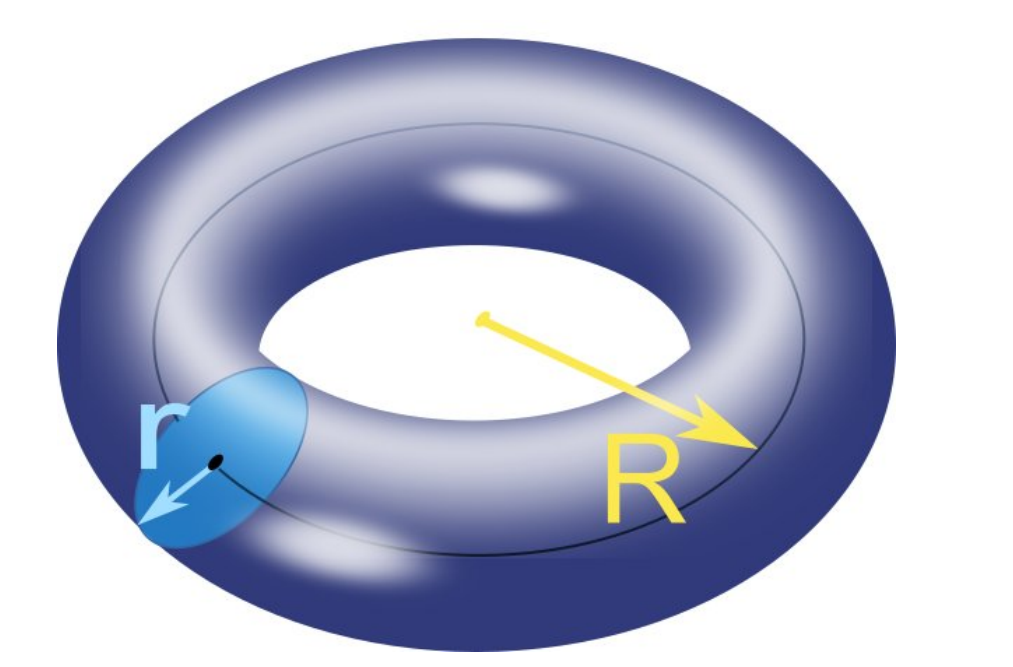
\includegraphics[width=\textwidth]{img/torus.png}
\end{subfigure}%
\begin{subfigure}{.5\textwidth}
    \centering
    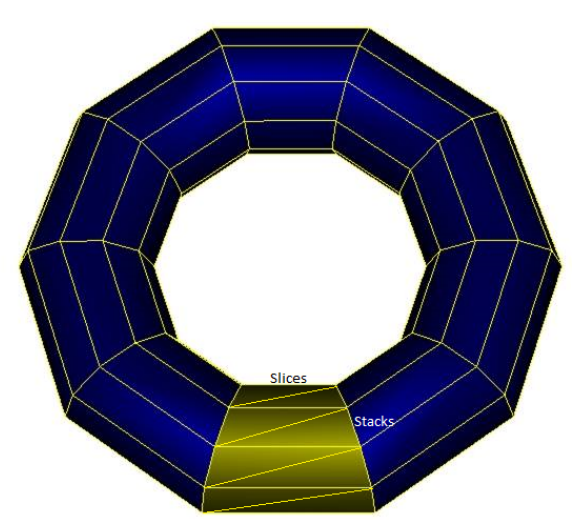
\includegraphics[width=\textwidth]{img/torus_1.png}
\end{subfigure}
\caption{Geometria de um \textit{torus}}
\end{figure}

\subsection*{Algoritmo}

Começamos um raio interno, de forma a definir a espessura do \textit{torus}, sendo
que a lateral pode ser dividida em \textit{stacks} e \textit{slices}. Desta forma,
começa-se por geral um anel, sendo este replicado até se completar o conjunto de
\textit{slices}. O raio exterior, por sua vez, define a abertura do \textit{torus},
ou seja, a distância entre os anéis e a origem do referencial.

De maneira a percorrer as circunferências, são utilizados os parâmetros \texttt{slices}
e \texttt{stacks} para dividir a execução em diferentes partes com amplitudes
\texttt{theta\_shift} e \texttt{phi\_shift}.

\

\begin{minted}{cpp}
float theta_shift = 2 * M_PI / slices;
float phi_shift = 2 * M_PI / stacks;
\end{minted}

\pagebreak

\begin{wrapfigure}{r}{.48\textwidth}
    \centering
    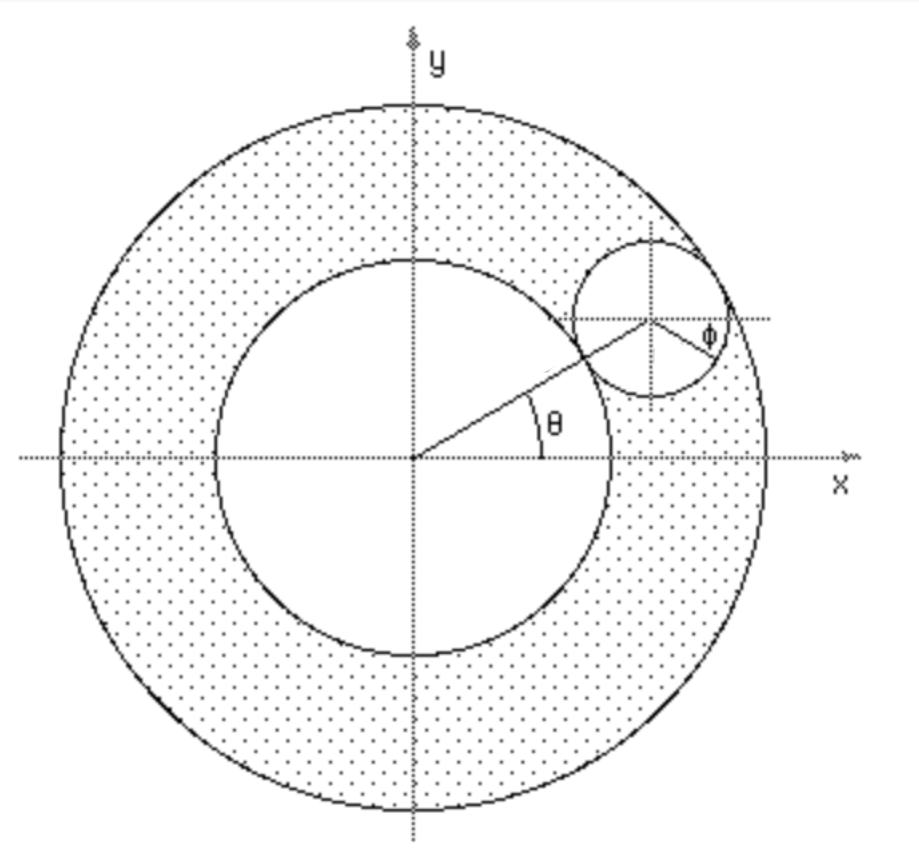
\includegraphics[width=.48\textwidth]{img/torus_2.png}
    \caption{Esquema de um \textit{Torus}}
    \label{fig:torus}
\end{wrapfigure}

Assim, é possível percorrer tanto a circunferência interna ao adicionar \texttt{phi\_shift},
como a externa ao adicionar \texttt{theta\_shift}. Note-se que as variáveis \texttt{theta}
e \texttt{phi} representam o ângulo interno e o externo, respetivamente, tal como
ilustrado na Figura \ref{fig:torus}. Portanto, foi criado um ciclo para a iteração
de cada circunferência. No final de cada iteração de construção de uma \textit{stack},
incrementa-se \texttt{phi} de maneira a formar um anel. Mas também, no final de
cada anel construído, incrementa-se o valor de \texttt{theta} de maneira a ser
possível a passagem para a construção do anel imediatamente a seguir ao que foi
gerado, até completar toda a circunferência externa e formar o \textit{torus}
pretendido.

\

\

O resultado da renderização pode ser visto na figura seguinte:

\begin{figure}[H]
    \centering
    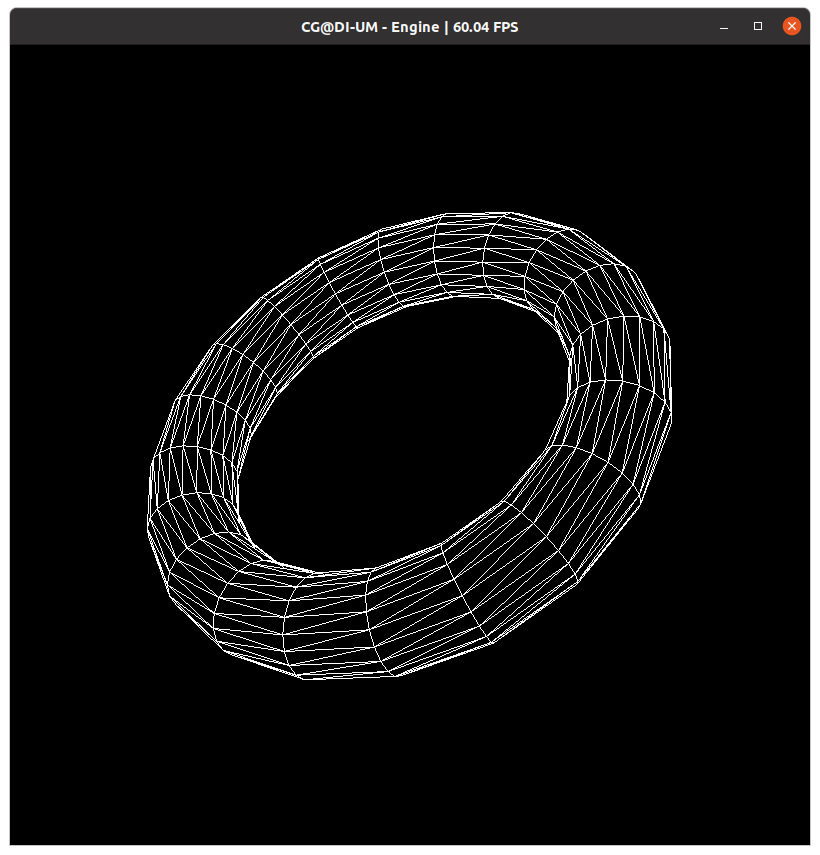
\includegraphics[width=.7\textwidth]{img/torus_3.png}
    \caption{\textit{Torus} com \textit{inner radius} 1, \textit{outer radius} 5,
    20 \textit{slices} e 20 \textit{stacks}, renderizado no modo \texttt{GL\_LINE}}
\end{figure}

\pagebreak

\section{\textit{Engine}}
\label{sec:engine}

Com o intuito de implementar as novas funcionalidades necessárias à realização
desta fase do trabalho prático, optamos por alterar a estrutura do código já elaborado.
Deste modo, criamos algumas classes, explicadas de seguida.

\subsection{Classe \textit{Transform}}

De modo a armazenar todas as informações relativas a uma transformação geométrica,
foi criada a seguinte classe \texttt{Transform}. As transformações geométricas podem
ser rotações, translações e escalas. Neste sentido, é necessário guardar o vetor
associado à transformação e, no caso de esta ser uma rotação, o ângulo.

\begin{minted}{cpp}
class Transform {
private:
    std::string type;
    float angle, x, y, z;
    // (...)
};
\end{minted}

\subsection{Classe \textit{Shape}}

A classe \texttt{Shape} é responsável por armazenar as coordenadas dos os vértices
necessários para representar uma determinada figura.

\begin{minted}{cpp}
class Shape {
private:
    std::vector<Vertex *> vertices;
    // (...)
};
\end{minted}

\subsection{Classe \textit{Group}}

A classe \texttt{Group} é responsável por armazenar toda a informação de um determinado
grupo, isto é, todas as informações relativas às primitivas geométricas e trasformações
associadas, sendo, por isso, uma das classes mais importantes do projeto. Esta armazena
todos os grupos filhos, assim como as transformações e as coordenadas pontos necessários
para desenhar cada uma das formas geométricas.

\begin{minted}{cpp}
class Group {
private:
    std::vector<Group *> groups;
    std::vector<Transform *> transforms;
    std::vector<Shape *> shapes;
    // (...)
};
\end{minted}

\subsection{Câmera}

Inicialmente, a câmera encontra-se orientada para a origem do referencial, sendo
esta capaz de se movimentar numa superfície esférica imaginária. Através da interação
com o teclado, é possível alterar o valor do raio desta superfície esférica imaginária,
assim como o valor dos ângulos $\alpha$ e $\beta$, que definem a posição da câmera.
Note-se que é também possível recolocar a câmera na posição inicial utilizando a tecla
\texttt{F3}.

De modo a implementar um menu que permite focar num determinado planeta, é necessário
garantir que o movimento da câmera acompanha a posição para a qual esta está a olhar.
Como tal, definimos as variáveis \texttt{look\_x}, \texttt{look\_y} e \texttt{look\_z},
que indicam a posição para a qual a câmera está virada. Assim, fazendo uso de
coordenadas esféricas, é possível definir a posição da câmera como:

\begin{minted}{cpp}
cam_x = look_x + radius * cos(beta) * sin(alpha);
cam_y = look_y + radius * sin(beta);
cam_z = look_z + radius * cos(beta) * cos(alpha);
\end{minted}

\begin{minted}{cpp}
class Camera {
private:
    float alpha, beta, radius;
    float cam_x, cam_y, cam_z;
    float look_x, look_y, look_z;
    // (...)
};
\end{minted}

\pagebreak

\section{\textit{Parser} e Processamento de ficheiros XML}

Nesta segunda fase do trabalho prático, existiu a necessidade de modificar a forma
como é efetuado o \textit{parsing} dos ficheiros XML uma vez que agora também é
necessário aplicar transformações geométricas às figuras obtidas através da leitura
dos ficheiros \texttt{.3d}. As informações relativas a estas transformações geométricas
encontram-se registadas nos ficheiros XML, daí ser necessário alterar o \textit{parser}.
À semelhança da primeira fase, para a leitura dos ficheiros XML, foi utilizada a
biblioteca \texttt{tinyxml2}, que disponibiliza um vasto conjunto de funções para o
tratamento deste tipo de ficheiros.

Um ficheiro XML é composto pelos seguintes elementos:

\begin{multicols}{2}
\begin{itemize}
    \item \textit{Scene};
    \item \textit{Group};
    \item \textit{Models};
    \item \textit{Rotate};
    \item \textit{Scale};
    \item \textit{Translate};
    \item \textit{Colour}.
\end{itemize}
\end{multicols}

\paragraph{\textit{Group}:} Determinados elementos e atributos podem ser agrupados
através do elemento \textit{group}.

\paragraph{\textit{Models}:} A \textit{tag} \textit{models} aparece associada aos
ficheiros \texttt{.3d}, que contêm as coordenadas dos vértices necessários à triangulação
de certas primitivas geométricas, necessárias para renderizar uma cena.

\paragraph{\textit{Rotate, Scale} e \textit{Translate}:} As \textit{tags} \textit{translate},
\textit{rotate} e \textit{scale} estão  associadas à translação, rotação e escala
de um determinado objeto, respetivamente.
 
\paragraph{\textit{Colour}:} De maneira a reconhecer os diferentes constituintes
do modelo do Sistema Solar, foi também utilizado um atributo que especifica a cor
dos mesmos. 

\

A seguir apresenta-se um exemplo da forma como estas \textit{tags} são utilizadas.

\begin{minted}{xml}
<group>
    <!-- Mercurio -->
    <translate X="-10" Z="20" />
    <scale X="0.24" Y="0.24" Z="0.24" />
    <colour R="0.2" G="0.2" B="0.2" />
    <models>
        <model file="sphere.3d" />
    </models>
</group>
\end{minted}

\hfill

\subsection*{\textit{Parsing}}

Inicialmente, o ficheiro XML é carregado para memória, utilizando a função 
\texttt{load\_XML\_file}, sendo esta responsável por invocar a função \texttt{parse\_group}
em caso de sucesso. Para tal, efetua-se um ciclo que percorre todos os nodos, processando
individualmente cada um deles. Caso este corresponda a uma transformação geométrica,
invoca-se a função responsável por recolher a informação necessária e adicioná-la
a uma estrutura de dados adequada. Note-se que as informações relativas à cor com a
qual as figuras deverão ser preenchidas vão também ser guardadas recorrendo à classe 
\texttt{Transform}, e, uma vez que estas estão também guardadas no ficheiro XML, irá ser 
necessário extraí-las juntamente com as informações das transformações geométricas. 

Por outro lado, o nodo poderá conter a informação do ficheiro \texttt{.3d} que deverá
ser lido. Nesse caso, é invocada a função \texttt{parse\_models}, que, por sua vez,
invoca a função \texttt{read\_file} com o intuito de ler as coordenadas dos pontos de
cada ficheiro, armazenando-os num vetor de formas geométricas, que será armazenado na
estrutura de dados principal.

\pagebreak

\section{Renderização do Modelo}

O \textit{engine} está dividido essencialmente em duas partes: a leitura do ficheiro XML,
e a interpretação e renderização do conteúdo do mesmo.

No que diz respeito à interpretação e renderização do conteúdo do ficheiro XML, na
função \texttt{renderScene} irá ser chamada a função \texttt{drawScene}, tendo esta
como único argumento o \texttt{Group} contendo toda a informação relativa ao modelo
do Sistema Solar. Antes de desenhar as primitivas, é necessário verificar não só
as transformações existentes, de forma a realizar as translações, rotações ou escalas
necessárias, mas também as aplicar a cor necessária à figura, tendo em conta os parâmetros
fornecidos para ambos os casos. Deste modo, fazendo uso das funções do openGl
(\texttt{glTranslatef}, \texttt{glRotatef}, \texttt{glScalef}, etc), a função \texttt{drawScene}
gera as respetivas figuras após aplicadas as devidas transformações geométricas.

Importa salientar que para o desenho em si, uma vez que serão efetuadas transformações
geométricas, existe uma alteração na matriz de transformação e por isso deve ser guardado
o estado inicial desta, e depois de todas as transformações serem aplicadas, este
estado deve ser reposto. Para isso são usadas as funções \texttt{glPushMatrix} e
\texttt{glPopMatrix} antes de aplicar a transformação e depois de esta ser aplicada, 
respetivamente. 

Depois de realizadas todas as transformações, percorre-se o vetor que contém as
coordenadas de todos os pontos necessários para desenhar as figuras e procede-se
ao desenho dos triângulos que as compõem usando a função \texttt{glBegin(GL\_TRIANGLES)}. 

Por fim, os grupos filhos são processados através de uma chamada recursiva à função
\texttt{drawScene}.

\pagebreak

\section{Sistema Solar}

Para a segunda fase do trabalho prático, foi proposta a elaboração de um modelo
estático do sistema solar, que contém o Sol, assim como os diferentes planetas e
respetivas luas. De modo a reaproveitar o trabalho realizado na primeira fase, foi
utilizado o ficheiro com o modelo da esfera para a representação de todos os elementos
do Sistema Solar. Assim, a esfera utilizada tem raio 5, 20 \textit{slices} e 20 \textit{stacks},
e o \textit{torus} tem \textit{inner radius} 1, \textit{outer radius} 5, 20 \textit{slices}
e 20 \textit{stacks}.

Para cada um dos corpos celestes foi escolhida uma cor e foi definida uma rotação
e translação de modo simular o movimento do planetas em torno do Sol. Foi também
atribuída uma escala de forma a simular o tamanho dos planetas.

Assim, tendo em consideração aspetos como o raio dos diferentes planetas ao Sol
e o seu raio, assim como a existência de anéis e satélites naturais, elaboramos um
ficheiro XML que permite a construção do modelo do Sistema Solar.

No entanto, ao tentar estabelecer uma escala realista, houve alguma dificuldade
uma vez que os últimos quatro planetas encontram-se muito distantes Sol, além de
que os satélites de cada um dos planetas são pequenos. Posto isto,
optamos por não fazer o Sistema Solar à escala, isto é, não respeitamos totalmente
as dimensões dos diferentes corpos celestes nem as distâncias que os separam, uma
vez que, caso o fizessemos, o resultado final seria um cenário muito disperso e de
difícil observação.

Após construção do modelo do Sistema Solar, foram obtidos os resultados que se
apresentam de seguida.

\begin{figure}[H]
    \centering
    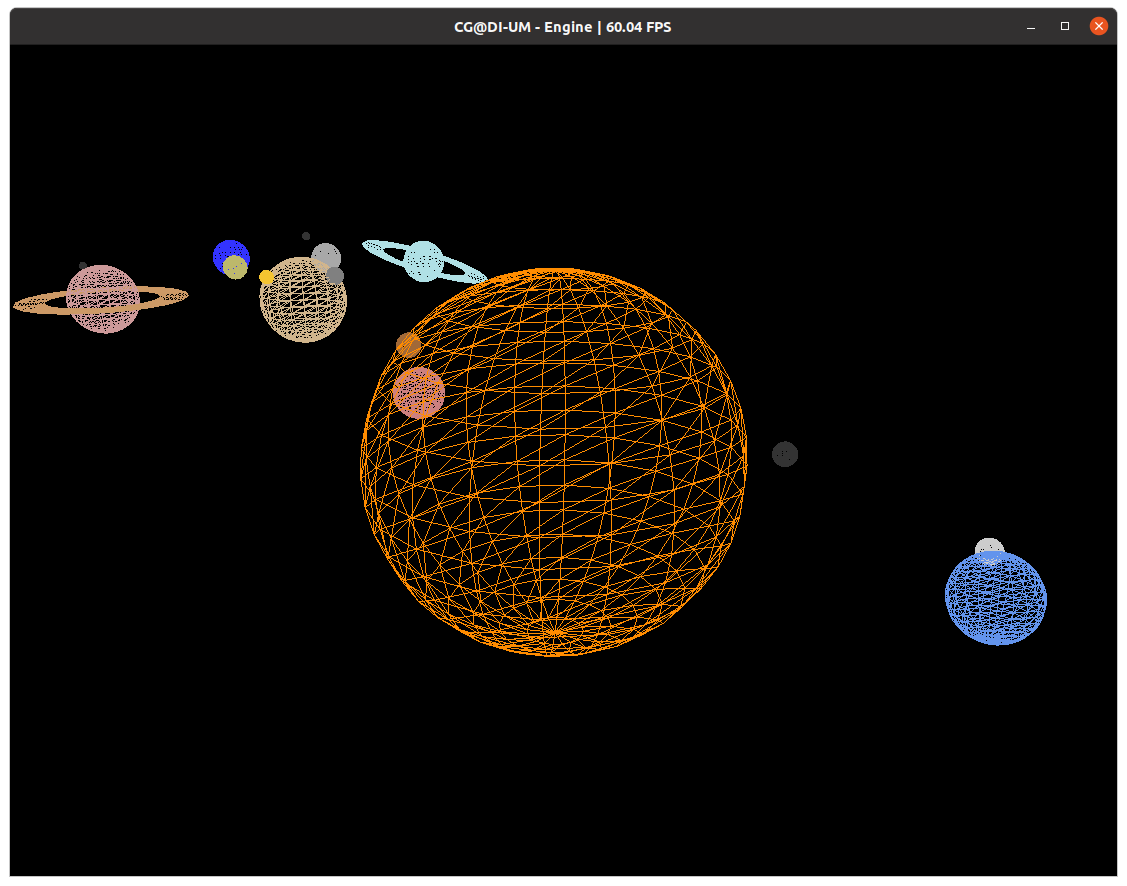
\includegraphics[width=.8\textwidth]{img/solarl.png}
    \caption{Modelo do Sistema Solar renderizado com linhas}
\end{figure}

\begin{figure}[H]
    \centering
    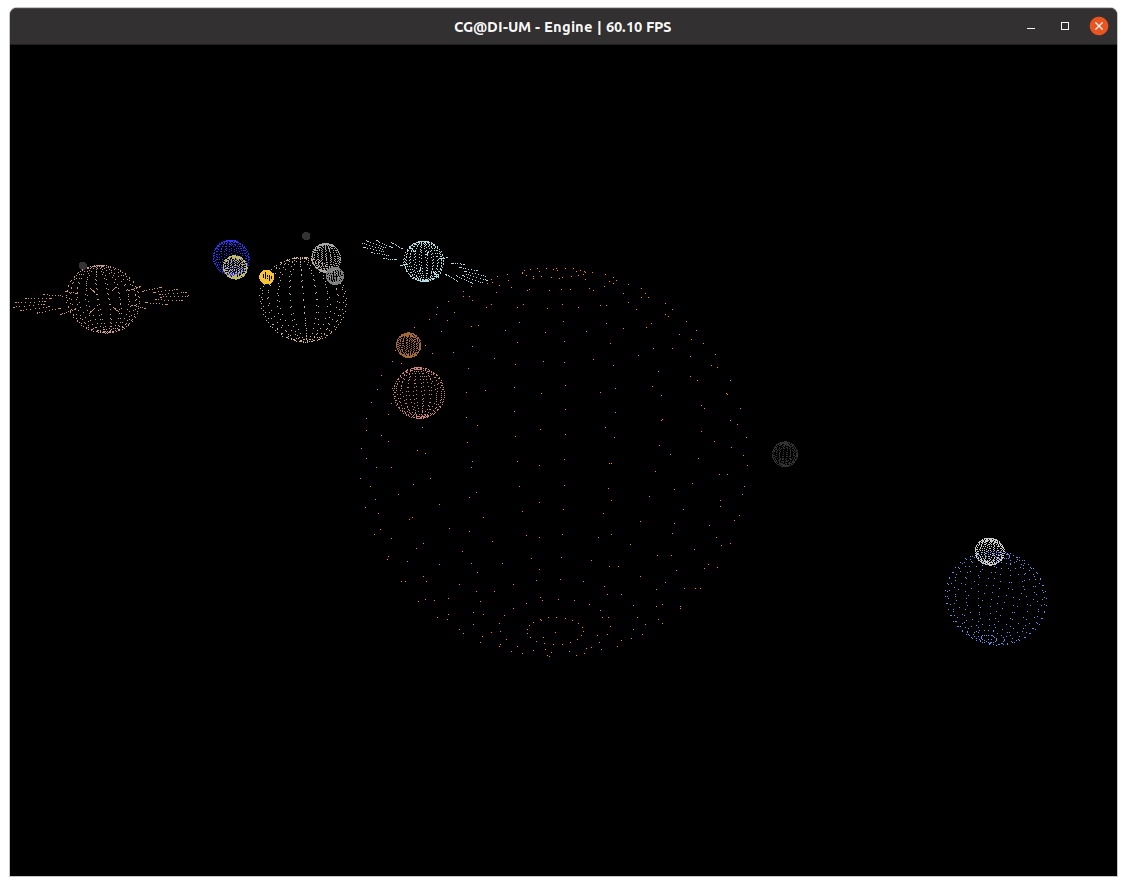
\includegraphics[width=.7\textwidth]{img/solarp.png}
    \caption{Modelo do Sistema Solar renderizado com pontos}
\end{figure}

\

\begin{figure}[H]
    \centering
    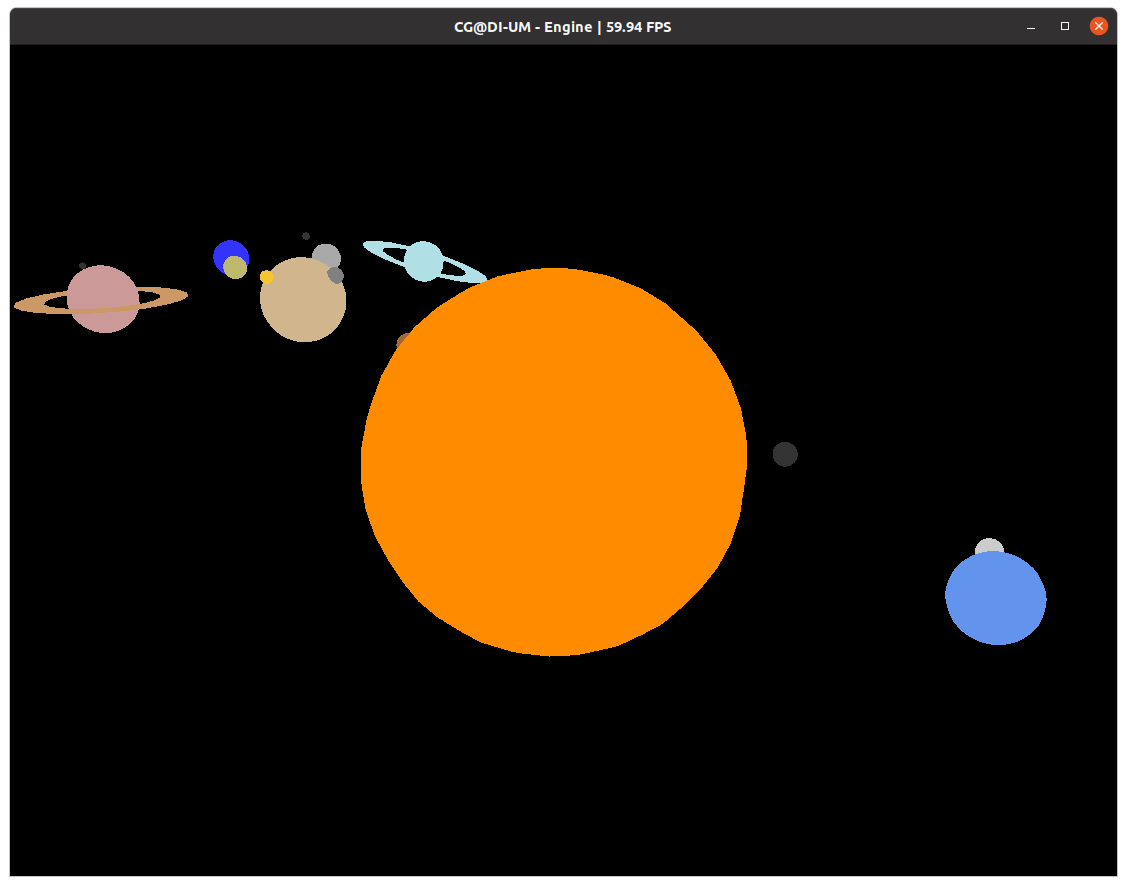
\includegraphics[width=.7\textwidth]{img/solarf.png}
    \caption{Modelo do Sistema Solar renderizado com as figuras preenchidas}
\end{figure}

\begin{figure}[H]
    \centering
    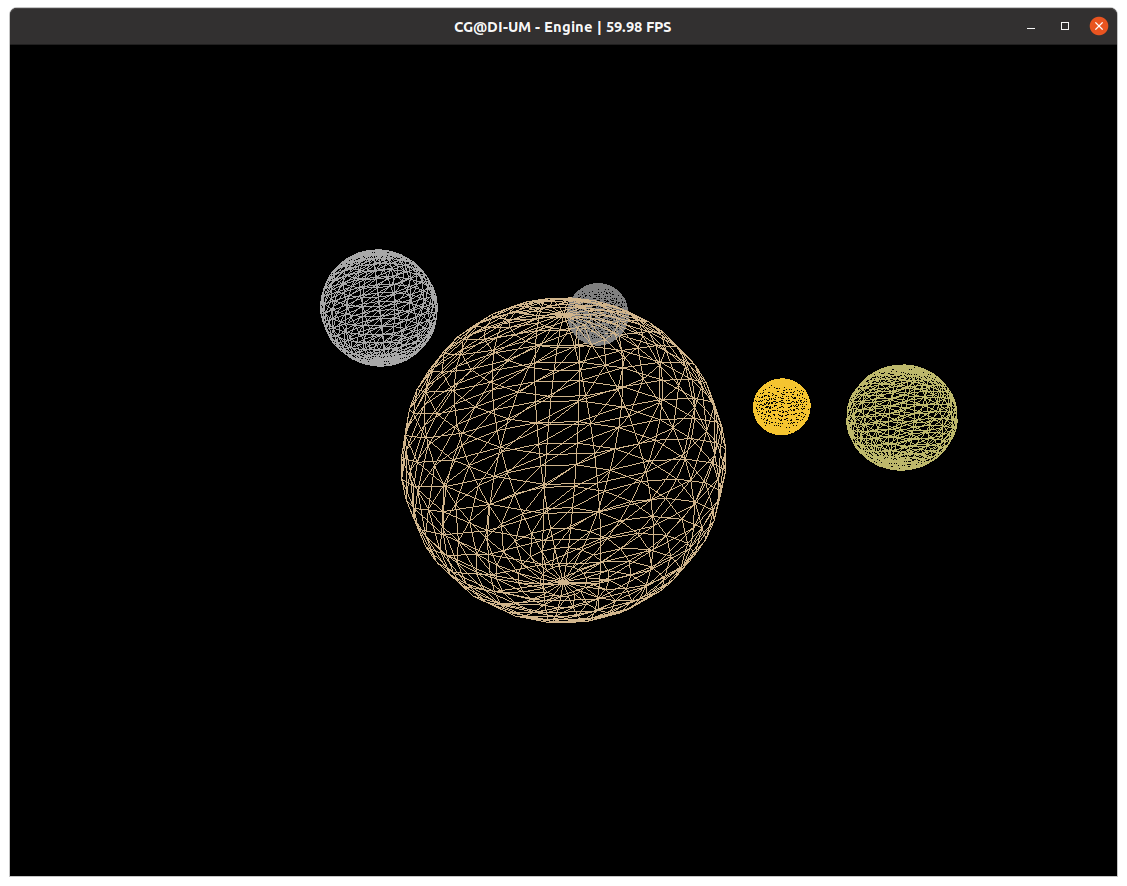
\includegraphics[width=.7\textwidth]{img/jupiter.png}
    \caption{Júpiter e os satélites IO, Europa, Calisto e Ganímedes}
\end{figure}

\

\begin{figure}[H]
    \centering
    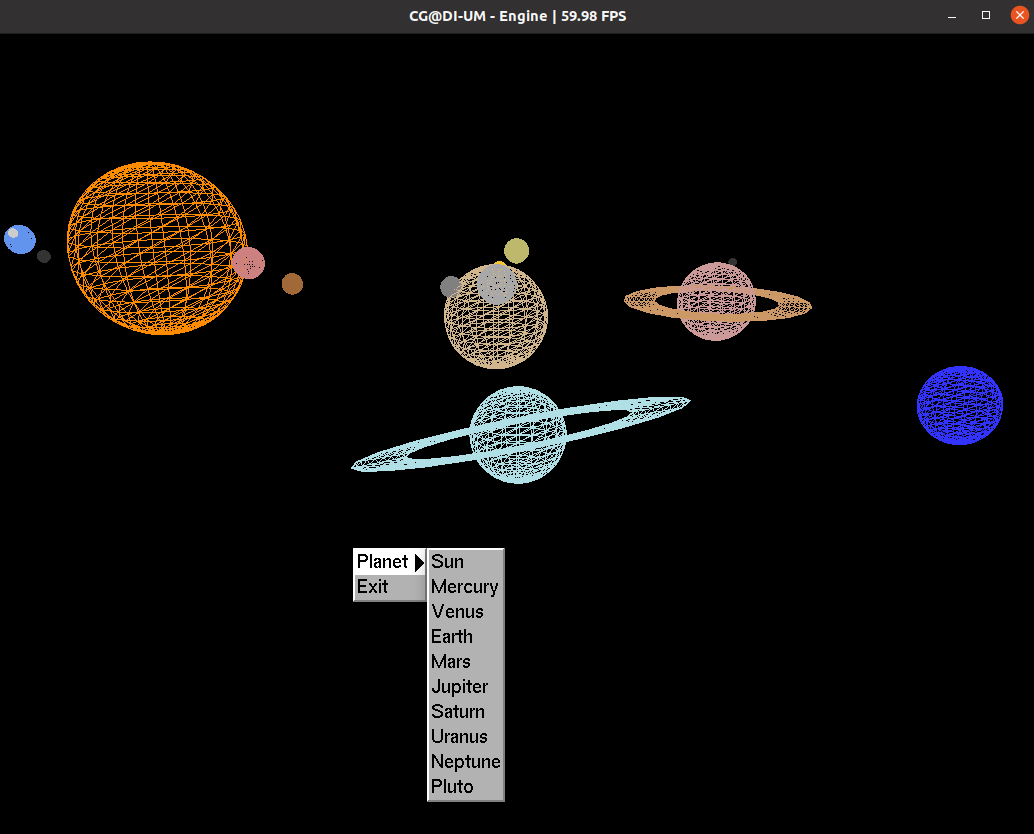
\includegraphics[width=.7\textwidth]{img/menu.png}
    \caption{Menu dos Planetas}
\end{figure}

\pagebreak

\section{Conclusão}

O desenvolvimento desta segunda fase do trabalho foi um pouco mais trabalhosa e
demorada em relação à primeira fase. Isto deve-se ao sobretudo à alteração da estrutura
dos ficheiros XML e consequentes alterações no \textit{parsing} destas informações.

Nesta segunda fase do trabalho prático foi-nos possível aprofundar e por em prática
conceitos relativos a transformações geométricas, o que nos permitiu ter uma melhor
noção da importância da ordem e do funcionamento base das mesmas. No geral, consideramos
que a maior parte dos resultados obtidos nesta fase correspondem aos esperado, uma vez
que apresentamos um modelo do Sistema Solar, ainda bastante simples mas com o objetivo de
nas fases que se seguem melhorar algumas questões. No entanto, ficaram por implementar alguns
aspetos, como por exemplo a cintura de asteróides e de \textit{Kuiper}.

Em conclusão, esperamos que nas restantes fases ultrapassemos estes obstáculos e consigamos
melhorar cada vez mais este modelo, tornando-o mais realista e mais apelativo visualmente.

\end{document}
